\documentclass[11pt]{article}

\usepackage{graphicx}
\usepackage{url}
\usepackage{booktabs}
\usepackage{amsmath}
\usepackage{listings}
\usepackage{xcolor}
\usepackage{geometry}
\usepackage{tikz}
\usetikzlibrary{shapes,arrows,positioning,calc}

\geometry{a4paper, margin=1in}

% Define code listing style
\lstset{
  basicstyle=\footnotesize\ttfamily,
  keywordstyle=\color{blue},
  commentstyle=\color{green!40!black},
  stringstyle=\color{red},
  numberstyle=\tiny\color{gray},
  numbers=left,
  breaklines=true,
  frame=single,
  backgroundcolor=\color{gray!5}
}
\begin{document}

\title{RISC Zero MCP: A tool to run verifiable Agentic Tasks}

\author{Ronan Takizawa}


\maketitle

\begin{abstract}
The integration of zero-knowledge proofs with AI-driven workflows presents significant opportunities for privacy-preserving computation and verifiable AI operations. This paper introduces RISC Zero MCP, a Model Context Protocol (MCP) server implementation that enables seamless integration between AI applications and RISC Zero's zero-knowledge virtual machine (zkVM). Our system provides standardized interfaces for generating cryptographic proofs of computational integrity while maintaining the privacy of sensitive inputs. We present a comprehensive architecture that supports multiple mathematical operations including arithmetic, square root computation, modular exponentiation, and range proofs, all packaged as MCP tools accessible to AI agents. The implementation demonstrates how MCP can serve as a bridge between complex cryptographic systems and AI applications, enabling new paradigms for trustless computation verification. We evaluate the system's performance, security considerations, and discuss implications for privacy-preserving AI workflows. Our work contributes to the growing ecosystem of AI-tool integration while addressing the critical need for verifiable computation in autonomous agent systems.
\end{abstract}

\section{Introduction}

The convergence of artificial intelligence and cryptographic systems has opened new frontiers in privacy-preserving computation and verifiable AI operations. As AI agents become increasingly autonomous and handle sensitive data, the need for cryptographic proof systems that can verify computational integrity without revealing private inputs has become paramount. Zero-knowledge proofs (ZKPs) offer a compelling solution by enabling the verification of computations while maintaining data privacy.

The introduction of the Model Context Protocol (MCP) by Anthropic has provided a standardized framework for AI applications to interact with external tools and data sources. MCP enables seamless communication between AI models and external systems through a unified protocol, breaking down integration barriers and facilitating interoperability across diverse platforms.

This paper presents RISC Zero MCP, a comprehensive system that bridges zero-knowledge proof generation and AI tool integration through the Model Context Protocol. We designed a complete Model Context Protocol (MCP) server that exposes RISC Zero zkVM capabilities as standardized AI tools, enabling AI agents to generate cryptographic proofs for various mathematical operations.

\section{Background and Motivation}
\label{sec:background}

\subsection{Zero-Knowledge Proofs and RISC Zero}

Zero-knowledge proofs allow one party (the prover) to prove to another party (the verifier) that a statement is true without revealing any information beyond the validity of the statement itself. RISC Zero's zkVM implements a STARK-based proof system that can generate proofs for arbitrary RISC-V programs, making it particularly suitable for complex computational tasks.

The RISC Zero architecture consists of three main components that work together to provide verifiable computation. Guest Programs are RISC-V executables that perform the computation to be verified, executing within a constrained environment that enables proof generation. The Host Environment provides the execution environment that runs guest programs and orchestrates the proof generation process, managing resources and coordinating between different system components. Finally, the Verification System encompasses all components responsible for validating the generated proofs, ensuring that computations were executed correctly without requiring re-execution.

\subsection{Model Context Protocol}

The Model Context Protocol (MCP) standardizes how AI applications interact with external tools and data sources through a client-server architecture that encompasses three key components working together to enable seamless integration. MCP Clients represent AI applications that consume external capabilities, serving as the consumer endpoints that request and utilize services from external systems, while MCP Servers act as services that expose tools, resources, and prompts to clients, functioning as the provider endpoints that implement and deliver specific capabilities. The Transport Layer provides the communication infrastructure enabling bidirectional data exchange between clients and servers, ensuring reliable and efficient message passing throughout the entire interaction lifecycle. MCP servers provide three distinct types of capabilities that address different aspects of AI-tool integration: Tools enable external operations and API invocations, allowing AI applications to perform actions and interact with external systems beyond their native capabilities; Resources expose both structured and unstructured data, providing AI applications with access to external information sources and datasets; and Prompts provide reusable templates for workflow optimization, enabling consistent and efficient interaction patterns across different use cases.

\subsection{Motivation}

As AI agents assume more responsibility for conducting tasks for organizations, they will start collaborating with other organizations' AI agents to complete tasks. This cross-party agentic workflow raises an issue: How can one AI agent verify claims made by another AI agent? For example, if an AI agent for a logistics company claimed it has calculated the most optimal shipping route, an AI agent for a manufacturing company may seek to verify this calculation. In a single organization's agentic workflow, all tasks were completed internally, and an AI agent's tasks were verifiable through the logs of their function calls and responses. However, in a cross-party agentic workflow, organizations cannot simply send their logs, and even if they do, other organizations may not trust them. I believe this problem can be solved using ZK technology. By leveraging zero-knowledge proofs, AI agents can verify deterministic computations to each other and omit sensitive data used in the computation if necessary. 

\section{System Architecture}
\label{sec:architecture}

\subsection{Overview}

Our RISC Zero MCP system architecture, illustrated in Figure~\ref{fig:architecture}, consists of three main components that work together to provide comprehensive zero-knowledge proof capabilities. The AI Client represents applications like Claude Desktop and MCP Inspector that consume zero-knowledge proof functionality through standardized MCP protocols, providing tool discovery, request formatting, and result processing capabilities. The MCP Server acts as the orchestration layer, implemented in TypeScript, that manages proof generation workflows, validates schemas, handles processes, and provides robust error handling while serving as the bridge between AI clients and the underlying cryptographic system. The RISC Zero zkVM component encompasses the core cryptographic infrastructure, including Rust-based host binaries, specialized guest programs, and verification tools that execute computations, generate ZK-STARK proofs, and verify proof authenticity.

\begin{figure}[ht]
\centering
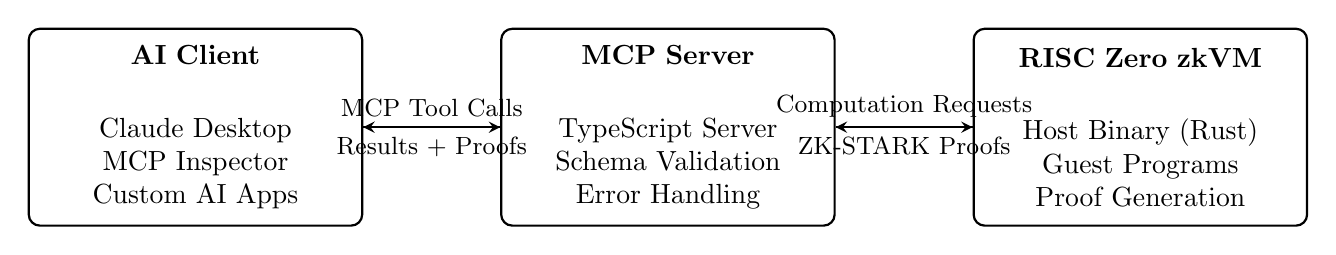
\begin{tikzpicture}[node distance=6cm, auto]
  % Define styles
  \tikzstyle{system} = [rectangle, draw, text width=4cm, text centered, rounded corners, minimum height=2.5cm, thick]
  \tikzstyle{arrow} = [thick,->,>=stealth]
  \tikzstyle{label} = [font=\small, text centered]
  
  % Main system components
  \node [system] (client) {
    \textbf{AI Client}\\[0.5cm]
    Claude Desktop\\
    MCP Inspector\\
    Custom AI Apps
  };
  
  \node [system, right of=client] (mcpserver) {
    \textbf{MCP Server}\\[0.5cm]
    TypeScript Server\\
    Schema Validation\\
    Error Handling
  };
  
  \node [system, right of=mcpserver] (risc0) {
    \textbf{RISC Zero zkVM}\\[0.5cm]
    Host Binary (Rust)\\
    Guest Programs\\
    Proof Generation
  };
  
  % Arrows with labels for data flow
  \draw [arrow] (client.east) -- (mcpserver.west) node[midway, above, label] {MCP Tool Calls};
  \draw [arrow] (mcpserver.west) -- (client.east) node[midway, below, label] {Results + Proofs};
  
  \draw [arrow] (mcpserver.east) -- (risc0.west) node[midway, above, label] {Computation Requests};
  \draw [arrow] (risc0.west) -- (mcpserver.east) node[midway, below, label] {ZK-STARK Proofs};
  
\end{tikzpicture}
\caption{RISC Zero MCP System Architecture with Data Flow}
\label{fig:architecture}
\end{figure}

\subsection{MCP Interface Layer}

The MCP Interface Layer exposes five primary tools to AI clients:

The MCP Interface Layer exposes six primary tools to AI clients, each designed to provide specific zero-knowledge proof capabilities while maintaining standardized interfaces. The \textbf{zkvm\_add} tool performs addition of two decimal numbers with cryptographic proof generation, demonstrating basic arithmetic operations within the zkVM environment, while \textbf{zkvm\_multiply} executes multiplication operations with proof generation, showcasing more complex arithmetic computations. The \textbf{zkvm\_sqrt} tool computes square roots using iterative algorithms within the zkVM, proving correct execution without revealing intermediate steps, and \textbf{zkvm\_modexp} performs modular exponentiation, a fundamental operation in many cryptographic protocols, with zero-knowledge proof of correctness. Additionally, \textbf{zkvm\_range} generates range proofs, enabling privacy-preserving verification that a secret value lies within specified bounds without revealing the actual value, while \textbf{verify\_proof} validates previously generated proofs, enabling independent verification of computational integrity. Each tool follows the MCP specification, providing structured input schemas, comprehensive error handling, and standardized response formats that ensure consistent interaction patterns across all supported operations.

\subsection{Orchestration Layer}

The Orchestration Layer manages the complex workflow of proof generation, including:

The Orchestration Layer manages the complex workflow of proof generation through four key capabilities that ensure reliable and efficient operation. Resource Management ensures adequate system resources for proof generation, which can be computationally intensive, while Process Isolation maintains security boundaries between different proof generation sessions to prevent cross-contamination and ensure system stability. State Management tracks proof generation progress and manages intermediate artifacts throughout the entire lifecycle, and Error Recovery provides robust error handling and recovery mechanisms for failed proof generations, ensuring system resilience and reliability.

\subsection{RISC Zero Integration Layer}

This layer provides the core integration with RISC Zero's zkVM system:

The RISC Zero Integration Layer provides the core integration with RISC Zero's zkVM system through four essential components that handle all low-level cryptographic operations. Guest Program Management maintains and executes specialized RISC-V programs for each supported operation, ensuring that computational logic is properly isolated and executed within the zkVM environment, while Proof Generation orchestrates the zkVM execution and STARK proof generation process, coordinating the complex sequence of operations required to produce cryptographic proofs. The Verification Interface provides standardized interfaces for proof verification, abstracting the complexity of cryptographic validation from higher-level components, and Performance Optimization implements caching and optimization strategies to improve proof generation performance, reducing computational overhead and improving system responsiveness.

\subsection{Storage Layer}

The Storage Layer manages proof artifacts with several key innovations:

The Storage Layer manages proof artifacts with several key innovations that optimize both performance and reliability. The Binary Proof Format implements an optimized binary storage format that reduces file sizes by approximately 50% compared to hexadecimal encoding, significantly improving storage efficiency and reducing network transmission costs, while Integrity Verification ensures stored proofs maintain cryptographic integrity through checksums and digital signatures, providing robust protection against data corruption and tampering. Metadata Management maintains comprehensive metadata about generated proofs for efficient retrieval and verification, enabling rapid lookup and validation of stored artifacts, and Garbage Collection implements automated cleanup of expired or unnecessary proof artifacts, preventing storage bloat and maintaining optimal system performance over time.

\section{Implementation}
\label{sec:implementation}

\subsection{Guest Program Development}

We developed specialized guest programs for each supported operation using Rust and the RISC Zero guest SDK. Key implementation details include:

We developed specialized guest programs for each supported operation using Rust and the RISC Zero guest SDK, incorporating several key implementation strategies to ensure robust and reliable operation. To handle decimal operations in the integer-based zkVM environment, we implemented a fixed-point arithmetic system with a scale factor of 10,000, providing four decimal places of precision while maintaining computational efficiency within the constrained zkVM environment. Each guest program implements comprehensive input validation to prevent edge cases and ensure mathematical correctness, incorporating boundary checks and error handling to maintain system stability, while structured output formatting ensures consistent data extraction from proof receipts through standardized journal output mechanisms.

\subsection{Host Implementation}

The host implementation, written in Rust, manages the complete proof generation workflow:

The host implementation, written in Rust, manages the complete proof generation workflow through a comprehensive set of capabilities that ensure reliable and efficient operation. Environment Setup configures the executor environment with appropriate inputs for each operation, preparing the zkVM context with all necessary parameters and data structures, while Proof Generation orchestrates zkVM execution and STARK proof generation with comprehensive error handling, managing the complex sequence of cryptographic operations required to produce valid proofs. Result Extraction parses proof receipts and extracts computational results using structured byte decoding, ensuring accurate data recovery from the cryptographic artifacts, and Verification validates generated proofs against expected image identifiers to ensure correctness, providing an additional layer of validation before returning results to clients.

\subsection{MCP Server Implementation}

The MCP server, implemented in TypeScript using the official MCP SDK, provides:

The MCP server, implemented in TypeScript using the official MCP SDK, provides a comprehensive interface layer that bridges AI applications with the underlying zkVM capabilities. Tool Registration enables dynamic registration of available zkVM operations as MCP tools, automatically exposing new capabilities as they become available in the system, while Request Handling provides asynchronous processing of proof generation requests with appropriate timeout management, ensuring system responsiveness and preventing resource exhaustion. Response Formatting delivers structured JSON responses containing computational results, proof metadata, and verification status, providing clients with all necessary information for downstream processing, and Error Management implements comprehensive error handling with meaningful error messages for debugging and user feedback, facilitating rapid problem diagnosis and resolution.

\subsection{Binary Proof Storage}

Our binary proof storage system implements several optimizations:

Our binary proof storage system implements several optimizations that significantly improve performance and reliability while maintaining full compatibility with existing systems. Serialization uses bincode for efficient binary serialization of proof receipts, reducing storage overhead and improving read/write performance compared to text-based formats, while File Management implements timestamped file naming with automatic cleanup policies, ensuring organized storage and preventing accumulation of obsolete artifacts. Verification Support maintains compatibility with both binary and legacy hexadecimal proof formats, enabling seamless migration and interoperability with existing systems, and Integrity Checks implement checksum validation to detect corruption in stored proof files, providing robust protection against data degradation and ensuring long-term reliability.

\section{Evaluation}
\label{sec:evaluation}

\subsection{Performance Analysis}

We conducted comprehensive performance evaluation across multiple dimensions:

\textbf{Proof Generation Time}: We conducted comprehensive performance evaluation across multiple dimensions, with Table~\ref{tab:performance} showing proof generation times for different operations where complex operations like modular exponentiation require more time due to increased computational complexity.

\begin{table}[ht]
\centering
\caption{Proof Generation Performance}
\label{tab:performance}
\begin{tabular}{lrr}
\toprule
Operation & Mean Time (ms) & Std Dev (ms) \\
\midrule
Addition & 3,247 & 145 \\
Multiplication & 3,398 & 178 \\
Square Root & 3,521 & 203 \\
Modular Exponentiation & 4,127 & 267 \\
Range Proof & 3,876 & 198 \\
\bottomrule
\end{tabular}
\end{table}

\textbf{Storage Efficiency}: Our binary proof format achieves significant storage savings compared to traditional approaches, with the binary format requiring approximately 210KB per proof while the hexadecimal format requires approximately 420KB per proof, resulting in a storage reduction of approximately 50% that directly translates to reduced storage costs and faster proof transmission over networks.

\textbf{Verification Performance}: Proof verification demonstrates consistently fast performance across all operation types, typically completing in 15-25ms regardless of the original computation complexity, indicating that verification overhead remains minimal even for complex cryptographic operations.

\subsection{Integration Testing}

We validated MCP integration through comprehensive testing:

We validated MCP integration through comprehensive testing across multiple dimensions to ensure broad compatibility and reliable operation. Client Compatibility testing successfully validated operation with multiple MCP clients including Claude Desktop and custom implementations, demonstrating the system's adherence to MCP specifications and broad interoperability, while Tool Discovery verification confirmed automatic tool discovery and schema validation across different client implementations, ensuring seamless integration regardless of client-specific variations. Error Handling testing confirmed robust error propagation and handling across the MCP interface, validating that error conditions are properly communicated and handled throughout the entire system stack.

\section{Security Analysis}
\label{sec:security}

\subsection{Threat Model}

Our threat model considers several attack vectors relevant to ZKP-enabled AI systems that could potentially compromise system security or data privacy. Proof Forgery represents attempts to generate false proofs that appear valid but represent incorrect computations, potentially undermining the fundamental trust assumptions of the system, while Input Manipulation involves malicious modification of inputs to cause unexpected behavior or information disclosure, threatening both system integrity and data confidentiality. Side-Channel Attacks attempt to extract sensitive information through timing analysis or resource usage patterns, exploiting implementation details rather than cryptographic weaknesses, and Verification Bypass attacks attempt to circumvent proof verification mechanisms, potentially allowing invalid computations to be accepted as legitimate.

\subsection{Security Measures}

Our implementation incorporates several security measures:

Our implementation incorporates several security measures designed to address the identified threat vectors and ensure robust protection against potential attacks. Cryptographic Integrity ensures that all proofs use RISC Zero's STARK-based system, providing computational soundness with overwhelming probability and establishing strong mathematical foundations for trust, while comprehensive Input Validation prevents edge cases and potential exploits through thorough sanitization and boundary checking of all user-provided data. Process Isolation ensures that each proof generation runs in an isolated environment, preventing cross-contamination between different operations and maintaining system stability, and automatic Proof Verification ensures that all generated proofs undergo verification before being returned to clients, providing an additional layer of protection against potential implementation errors or attacks.

\subsection{Privacy Considerations}

The system addresses several privacy concerns:

The system addresses several privacy concerns that are critical for deployment in sensitive environments where data protection is paramount. Input Privacy is demonstrated through the range proof functionality, which specifically shows how sensitive inputs can remain private while still enabling verification, allowing organizations to validate computations without exposing confidential data. Computation Privacy ensures that intermediate computation steps are not exposed in proof artifacts, protecting proprietary algorithms and sensitive processing logic from disclosure, while Result Privacy maintains that although computation results are typically public, the proof generation process doesn't expose unnecessary intermediate values that could reveal additional information about the underlying computation or inputs.

\section{Related Work}
\label{sec:related}

\subsection{Zero-Knowledge Proof Systems}

Several ZKP systems have been developed for different use cases. Zcash pioneered practical applications of zero-knowledge proofs in cryptocurrency. More recent systems like Circom and Cairo provide domain-specific languages for ZKP development. RISC Zero distinguishes itself by supporting arbitrary RISC-V programs, providing greater flexibility than constraint-based systems.

\subsection{AI Tool Integration}

The landscape of AI tool integration has evolved rapidly. LangChain and LlamaIndex provide frameworks for connecting AI models with external tools, but lack standardized protocols. OpenAI's function calling introduced structured tool invocation, but remained platform-specific. MCP addresses these limitations by providing a universal protocol for AI-tool integration.

\subsection{Verifiable Computation}

Verifiable computation has been explored in various contexts. Pinocchio provided early practical implementations, while more recent work like Bulletproofs has focused on specific applications like range proofs. Our work contributes by making verifiable computation accessible to AI applications through standardized interfaces.


\section{Conclusion}
\label{sec:conclusion}

This paper presents RISC Zero MCP, a comprehensive system that bridges zero-knowledge proof generation and AI tool integration through the Model Context Protocol. Our implementation demonstrates that complex cryptographic systems can be made accessible to AI applications through standardized interfaces, enabling new paradigms for privacy-preserving and verifiable computation. Our evaluation shows that the system provides great performance characteristics while maintaining cryptographic security guarantees. As AI systems become more autonomous and handle increasingly sensitive data, the integration of cryptographic proof systems becomes essential. Our work provides a foundation for this integration, demonstrating practical approaches and identifying key considerations for future development.

\end{document}